%============================================================
%  Chapter 2 — Requirements Analysis
%============================================================
\chapter{Requirements Analysis}
\label{chap:requirements}

\section{Introduction}

This chapter presents a comprehensive requirements analysis for the Vulnerability Management System. We identify the system's actors, define both functional and non-functional requirements, present use case diagrams with detailed scenarios, and conclude with a project Gantt timeline.

\section{System Actors}

The VMS is designed for four distinct user roles, each with specific responsibilities and system privileges:

\begin{table}[H]
\centering
\caption{System Actors and Their Responsibilities}
\label{tab:actors}
\begin{tabularx}{\linewidth}{lX}
\toprule
\textbf{Actor} & \textbf{Description and Responsibilities} \\
\midrule
\textbf{Security Analyst} &
The primary user of the system. Responsible for importing Nessus scan results, classifying findings by severity, mapping findings to assets and application owners, initiating the Ollama AI remediation assistant, and monitoring SLA compliance dashboards. \\[6pt]
\textbf{System Administrator (Sysadmin)} &
Assigned findings on specific assets. Responsible for executing remediation steps, updating finding status through the lifecycle, and requesting risk acceptance for findings that cannot be remediated. Interacts with the Ollama AI for step-by-step patch guidance. \\[6pt]
\textbf{Manager} &
Monitors overall security posture through executive dashboards. Approves or rejects risk acceptance requests submitted by Sysadmins. Receives summary notifications on overdue findings and SLA breaches. \\[6pt]
\textbf{Administrator} &
Manages user accounts, roles, and system configuration. Configures SLA policies per severity level, manages asset and application records, and configures email notification templates and SMTP settings. \\
\bottomrule
\end{tabularx}
\end{table}

\section{Use Case Diagram}

\begin{figure}[H]
\centering
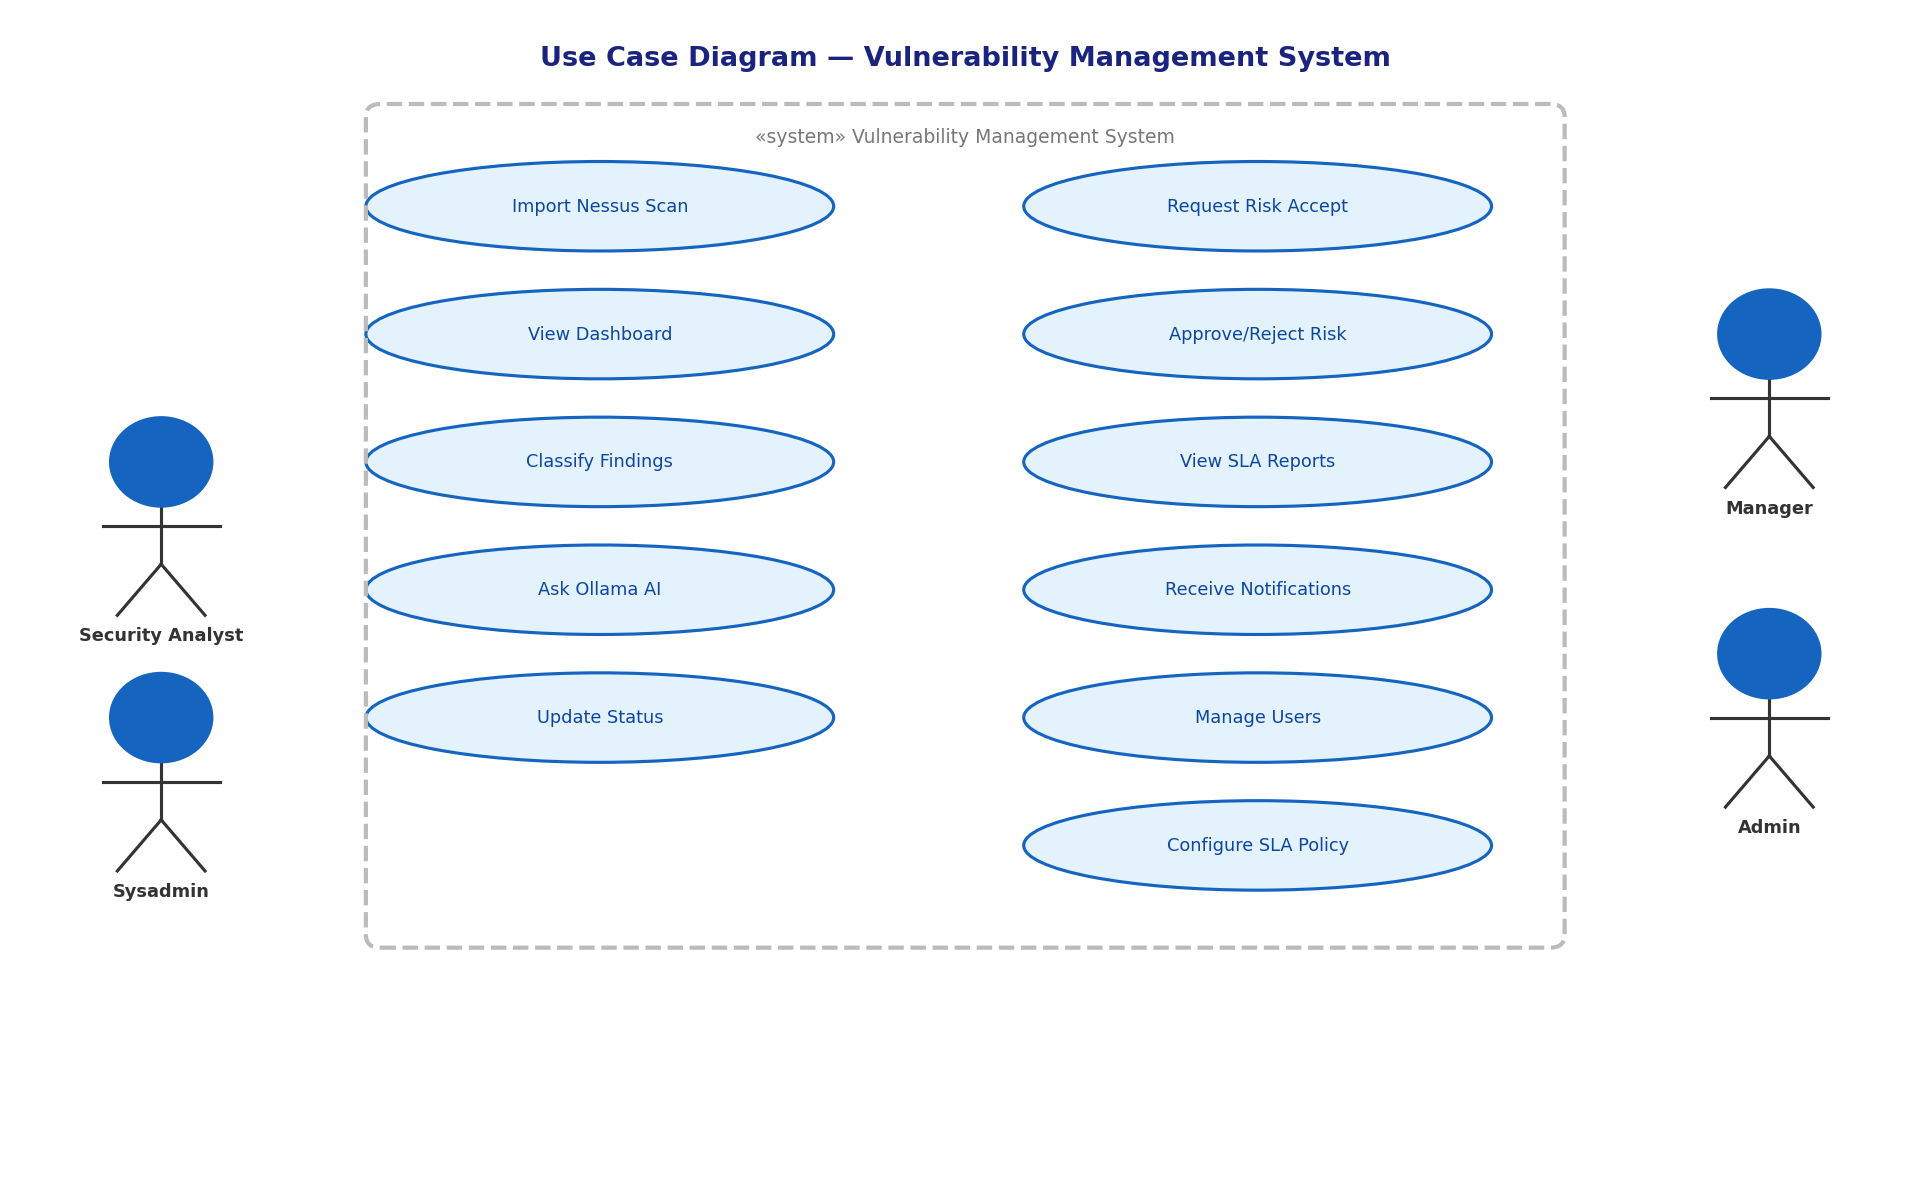
\includegraphics[width=0.95\linewidth]{img/usecase.png}
\caption{Use Case Diagram — Vulnerability Management System}
\label{fig:usecase}
\end{figure}

To complement the global use-case view in Figure~\ref{fig:usecase}, two additional UML diagrams were integrated to detail static and interaction perspectives of the system.

\begin{figure}[H]
\centering
\includegraphics[width=0.95\linewidth]{img/uml_static_structure.png}
\caption{UML Static Structure Diagram (User-Added)}
\label{fig:uml-static}
\end{figure}

\begin{figure}[H]
\centering
\includegraphics[width=0.95\linewidth]{img/uml_dynamic_interaction.png}
\caption{UML Dynamic Interaction Diagram (User-Added)}
\label{fig:uml-dynamic}
\end{figure}

Figures~\ref{fig:uml-static} and~\ref{fig:uml-dynamic} are used as supporting UML artifacts for the requirements phase and are referenced in the technical design chapter when discussing component interactions.

\section{Functional Requirements}

The following ten functional requirements define the core capabilities of the VMS:

\subsection{FR-01: Nessus Scan Import}
The system shall connect to the Tenable Nessus API using configurable credentials (API key and secret key) and import vulnerability findings in JSON format. The import process shall be triggerable manually via the web interface or schedulable as a background task.

\subsection{FR-02: Finding Deduplication}
The system shall deduplicate findings using a composite key composed of \texttt{(asset\_id, plugin\_id, port, protocol)}. When a finding matching an existing record is encountered, the system shall update the \texttt{last\_seen} timestamp rather than creating a duplicate entry.

\subsection{FR-03: Severity Classification}
The system shall classify findings into five severity levels based on Nessus plugin severity scores: Critical (CVSS $\geq$ 9.0), High (7.0--8.9), Medium (4.0--6.9), Low (0.1--3.9), and Informational (0.0). Each level shall have a distinct visual representation in the user interface.

\subsection{FR-04: SLA-Based Remediation Tracking}
The system shall calculate a remediation due date for each finding at import time, based on the finding's severity and the configured SLA policy. The system shall continuously monitor overdue findings and highlight them in the dashboard.

\begin{table}[H]
\centering
\caption{Default SLA Policy by Severity}
\label{tab:sla}
\begin{tabular}{lcc}
\toprule
\textbf{Severity} & \textbf{Remediation Window} & \textbf{CVSS Range} \\
\midrule
Critical & 7 calendar days & $\geq$ 9.0 \\
High & 15 calendar days & 7.0 -- 8.9 \\
Medium & 30 calendar days & 4.0 -- 6.9 \\
Low & 60 calendar days & 0.1 -- 3.9 \\
Informational & No deadline & 0.0 \\
\bottomrule
\end{tabular}
\end{table}

\subsection{FR-05: Finding Lifecycle Management}
The system shall support a multi-state finding lifecycle. Users shall be able to transition findings between states according to defined transition rules. The system shall log all status changes with timestamps and user attribution.

\subsection{FR-06: Risk Acceptance Workflow}
The system shall provide a formal risk acceptance process. Sysadmins may submit a risk acceptance request with a justification. Managers shall receive notification of pending requests and may approve or reject them via the web interface.

\subsection{FR-07: Ollama AI Remediation Assistant}
The system shall integrate with a locally deployed Ollama instance running the Mistral 7B model. For each finding, the system shall provide a chat interface where users can ask remediation questions. The AI shall receive full context including CVE details, severity, asset information, port, and protocol.

\subsection{FR-08: Email Notification System}
The system shall send automated email notifications for the following trigger events:
\begin{itemize}
  \item \textbf{ASSIGNED}: Finding assigned to a user
  \item \textbf{OVERDUE}: SLA deadline passed without remediation
  \item \textbf{HALF\_SLA}: 50\% of the SLA window consumed without progress
  \item \textbf{UNMAPPED\_FINDINGS}: Findings imported without asset/app mapping
  \item \textbf{RISK\_ACCEPTANCE\_REQUEST}: New risk acceptance awaiting manager review
\end{itemize}

\subsection{FR-09: Multi-Role Access Control}
The system shall enforce role-based access control. Each page and API endpoint shall verify the authenticated user's role before granting access. Unauthorized access attempts shall be redirected to an error page.

\subsection{FR-10: Dashboard and Reporting}
The system shall provide an executive dashboard displaying: total finding counts by severity, SLA compliance rate, overdue findings, recent findings table with filtering capabilities, and trend charts.

\section{Non-Functional Requirements}

\subsection{Performance}
\begin{itemize}
  \item Dashboard page load time: $< 2$ seconds (95th percentile)
  \item Nessus scan import: $< 60$ seconds for 500 findings
  \item Ollama first-token response: $< 3$ seconds on hardware with 8GB RAM
  \item API endpoint response time: $< 500$ms for read operations
\end{itemize}

\subsection{Scalability}
The system shall be designed to support up to 10,000 assets and 100,000 findings without architectural changes. Database queries shall use indexed columns for finding lookups.

\subsection{Security}
\begin{itemize}
  \item All user passwords shall be hashed using bcrypt with a cost factor $\geq 12$
  \item All API endpoints shall require session authentication
  \item CSRF protection shall be enabled for all state-changing operations
  \item Sensitive configuration (API keys, database passwords) shall be stored in environment variables, never in source code
  \item The Ollama endpoint shall not be exposed to external networks
\end{itemize}

\subsection{Reliability and Availability}
\begin{itemize}
  \item Target system availability: $\geq 99.5\%$ during business hours
  \item Email delivery success rate: $\geq 98\%$
  \item Database transactions shall be ACID-compliant
  \item Failed Nessus API calls shall be retried up to 3 times with exponential backoff
\end{itemize}

\subsection{Usability}
The web interface shall be responsive and functional on modern browsers (Chrome, Firefox, Edge). Bootstrap 5 shall be used for consistent, mobile-friendly layouts.

\section{Detailed Use Case Scenarios}

\subsection{UC-01: Import Nessus Scan}

\begin{table}[H]
\centering
\caption{Use Case: Import Nessus Scan}
\begin{tabularx}{\linewidth}{lX}
\toprule
\textbf{ID} & UC-01 \\
\textbf{Name} & Import Nessus Scan \\
\textbf{Actor} & Security Analyst \\
\textbf{Preconditions} & Nessus API credentials configured; user authenticated \\
\textbf{Main Flow} &
1. Analyst navigates to Import page \\&
2. System calls Tenable API to fetch latest scan results \\&
3. System iterates findings and checks composite key \\&
4. New findings are inserted; existing findings are updated \\&
5. System triggers notification for unmapped findings \\&
6. Import summary is displayed \\
\textbf{Alt. Flow} & If API returns error: system logs failure and displays error message \\
\textbf{Postconditions} & Finding database updated; import log created \\
\bottomrule
\end{tabularx}
\end{table}

\subsection{UC-02: Request Risk Acceptance}

\begin{table}[H]
\centering
\caption{Use Case: Request Risk Acceptance}
\begin{tabularx}{\linewidth}{lX}
\toprule
\textbf{ID} & UC-02 \\
\textbf{Name} & Request Risk Acceptance \\
\textbf{Actor} & Sysadmin \\
\textbf{Preconditions} & Finding exists in NEW or IN\_PROGRESS status \\
\textbf{Main Flow} &
1. Sysadmin opens finding detail page \\&
2. Clicks "Request Risk Acceptance" \\&
3. Enters justification and business reason \\&
4. System creates risk\_acceptances record (PENDING) \\&
5. System emails Manager with request details \\&
6. Finding status transitions to ACCEPTED\_RISK\_PENDING \\
\textbf{Alt. Flow} & Manager rejects: finding returns to IN\_PROGRESS \\
\textbf{Postconditions} & Risk acceptance record created; manager notified \\
\bottomrule
\end{tabularx}
\end{table}

\section{Project Gantt Diagram}

\begin{figure}[H]
\centering
\begin{tikzpicture}
\begin{axis}[
    xbar, xmin=0,
    width=0.92\linewidth, height=8cm,
    xlabel={Week Number},
    symbolic y coords={
      {Deployment \& Testing},
      {Chapter 4: Implementation},
      {Ollama Integration},
      {Notification System},
      {SLA Engine},
      {Chapter 3: Technical Design},
      {Database Schema},
      {Requirements Analysis},
      {Chapter 1-2: Analysis},
      {Environment Setup}
    },
    ytick=data,
    nodes near coords, nodes near coords align={horizontal},
    every node near coord/.append style={font=\tiny},
    enlarge y limits=0.1,
    bar width=8pt,
    grid=major,
    grid style={dashed, gray!30},
]
\addplot[fill=ISIblue!70] coordinates {
  (2,{Environment Setup})
  (3,{Chapter 1-2: Analysis})
  (3,{Requirements Analysis})
  (2,{Database Schema})
  (4,{Chapter 3: Technical Design})
  (2,{SLA Engine})
  (2,{Notification System})
  (3,{Ollama Integration})
  (4,{Chapter 4: Implementation})
  (3,{Deployment \& Testing})
};
\end{axis}
\end{tikzpicture}
\caption{Project Gantt Chart — Approximate Sprint Timeline (12 Weeks)}
\label{fig:gantt}
\end{figure}

\section{Summary}

This chapter defined all stakeholders, functional requirements, and non-functional constraints of the VMS. Ten functional requirements cover the complete vulnerability management lifecycle from import to closure, with particular emphasis on SLA enforcement, AI assistance, and risk acceptance workflows. The next chapter presents the detailed technical architecture implementing these requirements.
